\documentclass[12pt]{thesis} %%%%%%%%%%%%%%%%%%%%%%%%%%%%%%%%%%%%%%%%%%%%%%%%%%

%%% preample %%%%%%%%%%%%%%%%%%%%%%%%%%%%%%%%%%%%%%%%%%%%%%%%%%%%%%%%%%%%%%%%%%


%%% packages %%%%%%%%%%%%%%%%%%%%%%%%%%%%%%%%%%%%%%%%%%%%%%%%%%%%%%%%%%%%%%%%%%
% If the IEEEtran.cls has not been installed into the LaTeX system files,
% manually specify the path to it:
% \documentclass[conference]{../sty/IEEEtran}

\usepackage[T1]{fontenc}        % euro quality fonts [T1] (togeth. w/ textcomp)
\usepackage{textcomp, amssymb}  % additional symbols (there are more packages)
\usepackage[latin1]{inputenc}   % umlaute in input file
\usepackage{setspace}           % doublespacing
\usepackage{anysize}            % margin package sets tighter margins
\usepackage[all]{xy}            % creating figures within latex
\usepackage[tight]{subfigure}% subfigures: figures within figures
\usepackage{multirow}
\usepackage{url}
\usepackage{amsmath}
\usepackage{float}

\newcommand{\etal}{{\it et al.}}
\newcommand{\etc}{{\it etc.}}
\newcommand{\ie}{\emph{i.e.}}
\newcommand{\eg}{{\em e.g.}}
\newcommand{\msymb}[1]{\text{\it #1}}
\newcommand{\m}[1]{\mathcal{#1}}
\newcommand{\me}{BtrPlace}

%\marginsize{1.2in}{0.9in}{1.1in}{0.9in} % small margins
\marginsize{1.2in}{0.9in}{0.5in}{1.5in} % small margins

\usepackage{ifpdf}              % if pdflatex then ... else ...
\ifpdf
  \pdfadjustspacing=1           % make pdflatex behave like latex
  \usepackage{aeguill}          % PS converted CM fonts for better acro preview
  \usepackage[pdftex]{graphicx} % graphics packages
  \usepackage[pdftex]{color}    % color packages
  \usepackage[pdftex]{thumbpdf} % create thumbnails (run thumbpdf as well)
  \usepackage[pdftex,colorlinks,%
              pagebackref=true, % bibliography -> text
              linktocpage=true, % toc etc: make page number active (not name)
              plainpages=false, % distinguish roman and arabic pagenumbers
              bookmarksopen=true,%
              bookmarksnumbered=true,%
              pdfauthor={},%
              pdftitle={},% 
              pdfsubject={},%
              pdfkeywords={},%
             ]{hyperref}        % clickabe references
\else
  \usepackage[hypertex,
              plainpages=false, % distinguish roman and arabic pagenumbers
              linktocpage=true, % toc etc: make page number active (not name)
             ]{hyperref}        % clickabe references in .dvi
                                % purposely included before color package
  \usepackage[dvips]{color}     % color packages; needed by xy
  \usepackage[dvips]{graphicx}  % graphics packages
\fi


% hyperref must be the second last package and glossary the last package

% index
\usepackage{makeidx}                       % for \printindex
\makeindex                                 % creates paper.idx index file

% glossary
\usepackage[style=super, cols=3]{glossary} % for \printclossary
\makeglossary                              % creates paper.glo glossary file

%%% style and finetuning %%%%%%%%%%%%%%%%%%%%%%%%%%%%%%%%%%%%%%%%%%%%%%%%%%%%%%

\pagestyle{plain}               % pagestyle: headings, empty, plain

% new theorems
\newtheorem{example}{Example}
\newtheorem{proof}{Proof}


%%% document %%%%%%%%%%%%%%%%%%%%%%%%%%%%%%%%%%%%%%%%%%%%%%%%%%%%%%%%%%%%%%%%%%

\begin{document}

\pagenumbering{roman} % titlepage does not get a number - that's odd, but good.

\ifpdf\pdfbookmark[1]{Title}{label:title}\fi              % !TEX root =  thesis.tex

\thispagestyle{empty}%%%%%%%%%%%%%%%%%%%%%%%%%%%%%%%%%%%%%%%%%%%%%%%%%%%%%%%%%%


\begin{center}

\vspace*{\fill}
\noindent\rule{13cm}{2pt}\\[0.5cm]
{\huge \bf Multi-Agent System Simulator}
\noindent\rule{13cm}{2pt}\\[1cm]
\vspace*{\fill}
\par CISC475/675 Fall 2014 Team 6 \\
         Mike Boch \\ 
         Benjamin Gotthold\\ 
         Steven Noyes \\ 
         Varun Sharma \\
         Stefan Zimmerman \\






\vfill

% Bottom of the page
\date{\today}

\end{center}


%%%%%%%%%%%%%%%%%%%%%%%%%%%%%%%%%%%%%%%%%%%%%%%%%%%%%%%%%%%%%%%%%%%%%%%%%%%%%%%

\newpage
{Preliminaries}


\paragraph{Change Log}
\begin{itemize}
\item v0.4 10/31/2014 - In this release we continued to work on the requirements
document making images clearer, correcting spelling, and fixing formatting mistakes. We incorporated comprehensive coverage testing and created a verification plan to help improve our software accuracy. We were able to link the main modules of our program to provide the first runnable iteration where we created a simple external agent to assist in the running of a basic simulation. 
\item v0.3 10/17/2014 - Fixed several errors in the document in terms
of spelling and grammar. Updated the USES diagrams of the system and the tasktree package. Added detailed descriptions of the cTAEMS grammar and the task tree. Gave more detail on each stakeholder. Updated the ERD to reflect their proper language. Added descriptions of the interface that the Agents must adhere too. Added sample messages of each type for the Agents. Added an example task tree to show how a small scale simulation would run. Removed the cost attribute from the task tree. Updated the description of each module and package. Added a test verification plan. Converted most applicable images to the SVG format. Removed references to the Event Engine as it is no longer needed. Changed Event to Node as it fits the task tree design better. Added more detail to some of the Core Features. Added more terms to the Definition of Concepts.
\item v0.2 10/03/1014 - This release focused on clarifying the project
requirements and incorporating some basic design ideas. We worked to correct errors in the document pointed out by our client and instructor and added some additional content and figures. The most notable change is the addition of Chapter 5, Detailed System Design, where we began describing the transition from requirements to actual code.
\item v0.1 09/19/2014 - Initial Document Release
\end{itemize}


\paragraph{Team Information  \\ \\} 

This project, including the content of this document, have been designed by University of Delaware students Mike Boch, Ben Gotthold, Steven Noyes, Varun Sharma, and Stefan Zimmerman. To view the current release of this project please visit our project page at \color{black}\url{http://cisc475-6.cis.udel.edu}
.

\newpage                                                     %\input{spruch.tex}

{

}

\newpage\ifpdf\pdfbookmark[1]{Table of Contents}{label:toc}\fi \tableofcontents
\newpage\ifpdf\pdfbookmark[1]{List of Figures}{label:lof}\fi     \listoffigures

%
%
%
% THERE WAS AN OPEN BRACKET HERE THAT I GOT RIG OF BECUASE IT THREW AN ERROR-Ben
%
%
%
%

\newpage\pagenumbering{arabic}

% !TEX root =  thesis.tex
\chapter{Introduction}\label{chapter:introduction} %%%%%%%%%%%%%%%%%%%%%%%%%%%%


As technology advances, software is fast becoming the most economical way to test complex solutions to real world problems. Software testing allows a user to run unlimited iterations with complete control over environmental variables. Our Multi-Agent System Simulator (MASS) will provide an environment for Dr. Decker and other researchers to test software Agents allowing them to design more accurate solutions to real world problems faster than ever before.

\section{Document Purpose}

The purpose of this Software Requirements Specification (SRS) is to serve as a statement of understanding between the users of the proposed product and the software developers of the product. The Software Requirements Specification is defined using a subset of the Unified Modeling Language(UML), an Entity-Relationship Diagram(ERD) describing all of the objects/entities along with their attributes, relations, and Data Flow Diagram (DFD).

\section{Scope}

We will develop a general-purpose command line program called ?Multi-Agent System Simulator? (MASS). The MASS will take a Simulation File Input (SFI) and a Configuration File Input (CFI) to produce an environment in which user defined software Agents can connect and interact to solve problems. Upon completion the MASS will output the results of the problem Simulation as well as produce a Log File Output (LFO) detailing the events that occurred within the Simulation. The SFI will be a CTAEMS file describing the task domain that the MASS will use to construct the Simulation environment. The CFI will be a plain text file that contains settings relating to the execution of the MASS but are independent of a given SFI. Agents, which are independent user-defined programs, will connect to the MASS through TCP socket connections before a simulation begins. While running, the MASS allows inter-Agent communication and logs statistics such as the number of messages sent by each Agent. Upon completion the MASS will output the results of the simulation in terms of Quality, Cost, and Duration. It is important to note that the MASS does not restrict the design of the Agents themselves but requires them to adhere to an connection interface so that communication is possible.


\section{Acronyms and Abbreviations}

This section contains definitions of acronyms and abbreviations used in this document.

\begin{itemize}
\item{\textbf{MASS}: Multi-Agent System Simulator}
\item{\textbf{SFI}: Simulation File Input}
\item{\textbf{CFI}: Configuration File Input}
\item{\textbf{LFO}: Log File Output}
\item{\textbf{EE:} Event Engine}
\item{\textbf{UML}: Unified Modeling Language}
\item{\textbf{DFD}: Data Flow Diagram}
\item{\textbf{TCP:} Transmission Control Protocol}
\item{\textbf{JSON}: JavaScript Object Notation}
\item{\textbf{SRS}: Software Requirements Specification}
\item{\textbf{ERD}: Entity-Relationship Diagram}
\end{itemize}




\chapter{General Description}\label{chapter:general}

The product is meant to serve as a common platform for academic and research oriented activities in the area of Multi-Agent Simulation. The following sections describe the high level view of the system and establish its context. These sections do not state specific requirements but make the specific requirements easier to understand.

\section{Stakeholders}
The stakeholders of the Multi-Agent System Simulator are classified into the following categories.

\begin{itemize}
\item{\textbf{Dr. Decker}: Needs a platform to test his software agents in a way that can help advance his research and lead to new innovations. He can be contacted through email and met with in person readily.}

\item{\textbf{Dr. Siegel}: Needs a challenging project for his 475 students that is able to be completed over the course of the semester. The project should condone the use of software tools to test implementations and  track changes. He can be contacted through email or Skype and can be met with in person readily.}

\item{\textbf{Researchers}: Researchers might want to use this software for their research to design agents and simulations when testing new ideas.}

\item{\textbf{CIS faculty}: Needs an interactive tool for students to make the task of learning more interesting.}

\item{\textbf{Developers}: Developers are responsible for the designing, testing, configuring, and upgrading of the subsystems.}

\item{\textbf{Support}: Support personnel are responsible for the maintenance of the system, the software, the installation of subsystems, and configuration changes.}
\end{itemize}
% !TEX root =  thesis.tex
\chapter{General System Requirements}\label{systemRequirements}

The MASS is designed as a domain independent central process where all domain knowledge is obtained from the SFI and CFI. To prevent any interference or assumption, the MASS and the Agents run as separate independent processes. The cTAEMS model supplies the internal knowledge used to build a Task Tree from which Agents will select available Methods for execution. This coupled with the easy configuration mechanism, logging, reporting and statistical analysis makes the simulator a good platform for research and evaluation of Multi-Agent Systems.

\section{System Features}

The following list offers a brief outline and description of the main features and functionalities of the MASS. The features are split into two major categories: core features and optional features. Core features are essential to the application's operation, whereas optional features are preferred but not required. For a better understanding of the basic features of the system see Figure 3.1.
%~\ref{fig:ERD}

\begin{figure}[H]
\centering
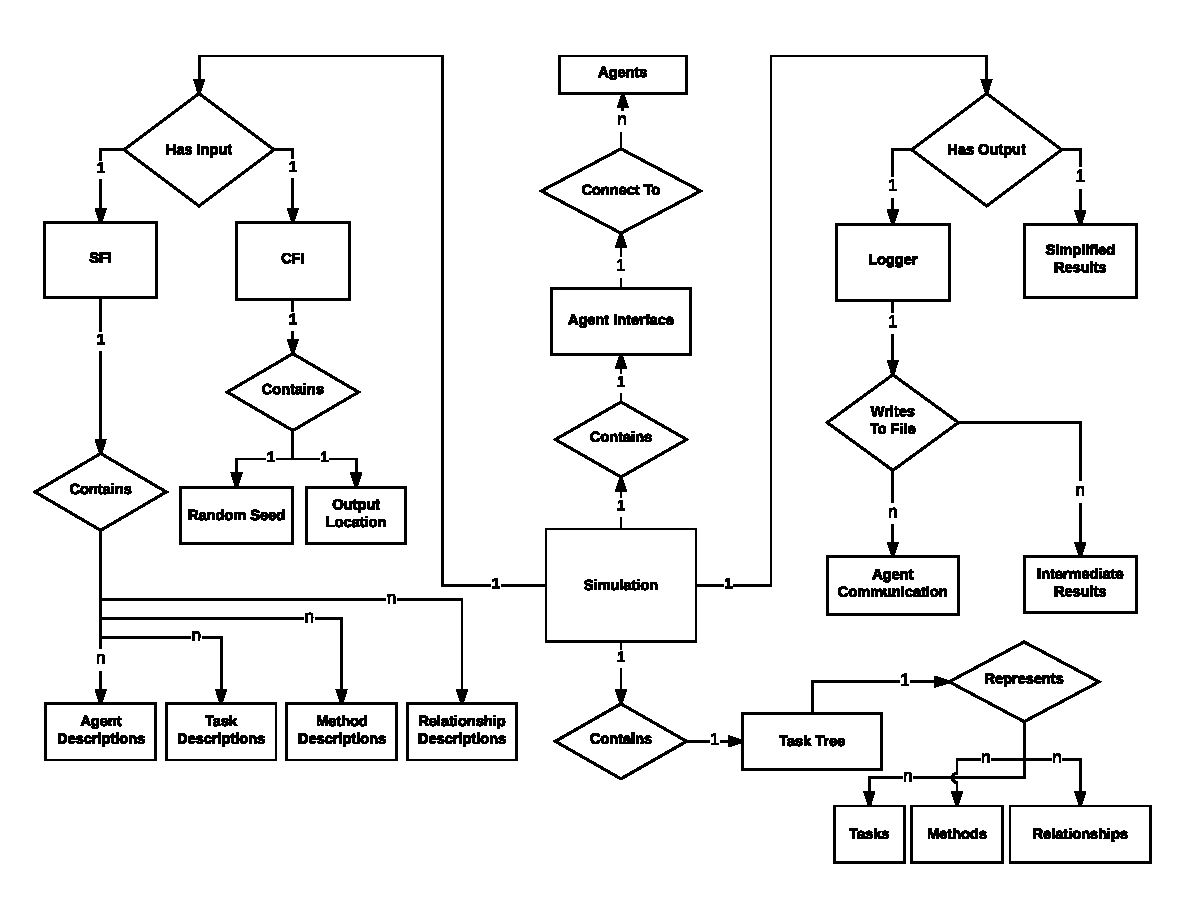
\includegraphics[width=6.5in]{figs/ERD.pdf}
\caption{ERD diagram for basic components of MASS.}
\label{fig:ERD }
\end{figure}

\begin{center} \textbf{Core Features} \end{center}


\begin{enumerate}

  \item\textbf{Running The MASS}: The MASS will run via the command line inside of a BASH script that takes the SFI and optionally the CFI as inputs.
  
  \item\textbf{Simulation File Input (SFI)}: The SFI is a cTAEMS file.
    \begin{enumerate}
    \item The system is only required to support the use of the AND, OR, and SUM QAFs of the cTAEMS grammar.
    \item Methods and Tasks may only have Qualities and Durations. Costs will not be implemented.
    \item The grammar of the cTAEMS file is in Figures 3.2 and 3.3(items in all capitals are variable).
    	\subitem QAF can be q\_and, q\_sum, or q\_or.
    	\subitem ENABLES\_DISABLES can be enables or disables.
    	\subitem FACILITATES\_HINDERS can be facilitates or hinders.
  \end{enumerate}
  
\begin{figure}[H]
\centering
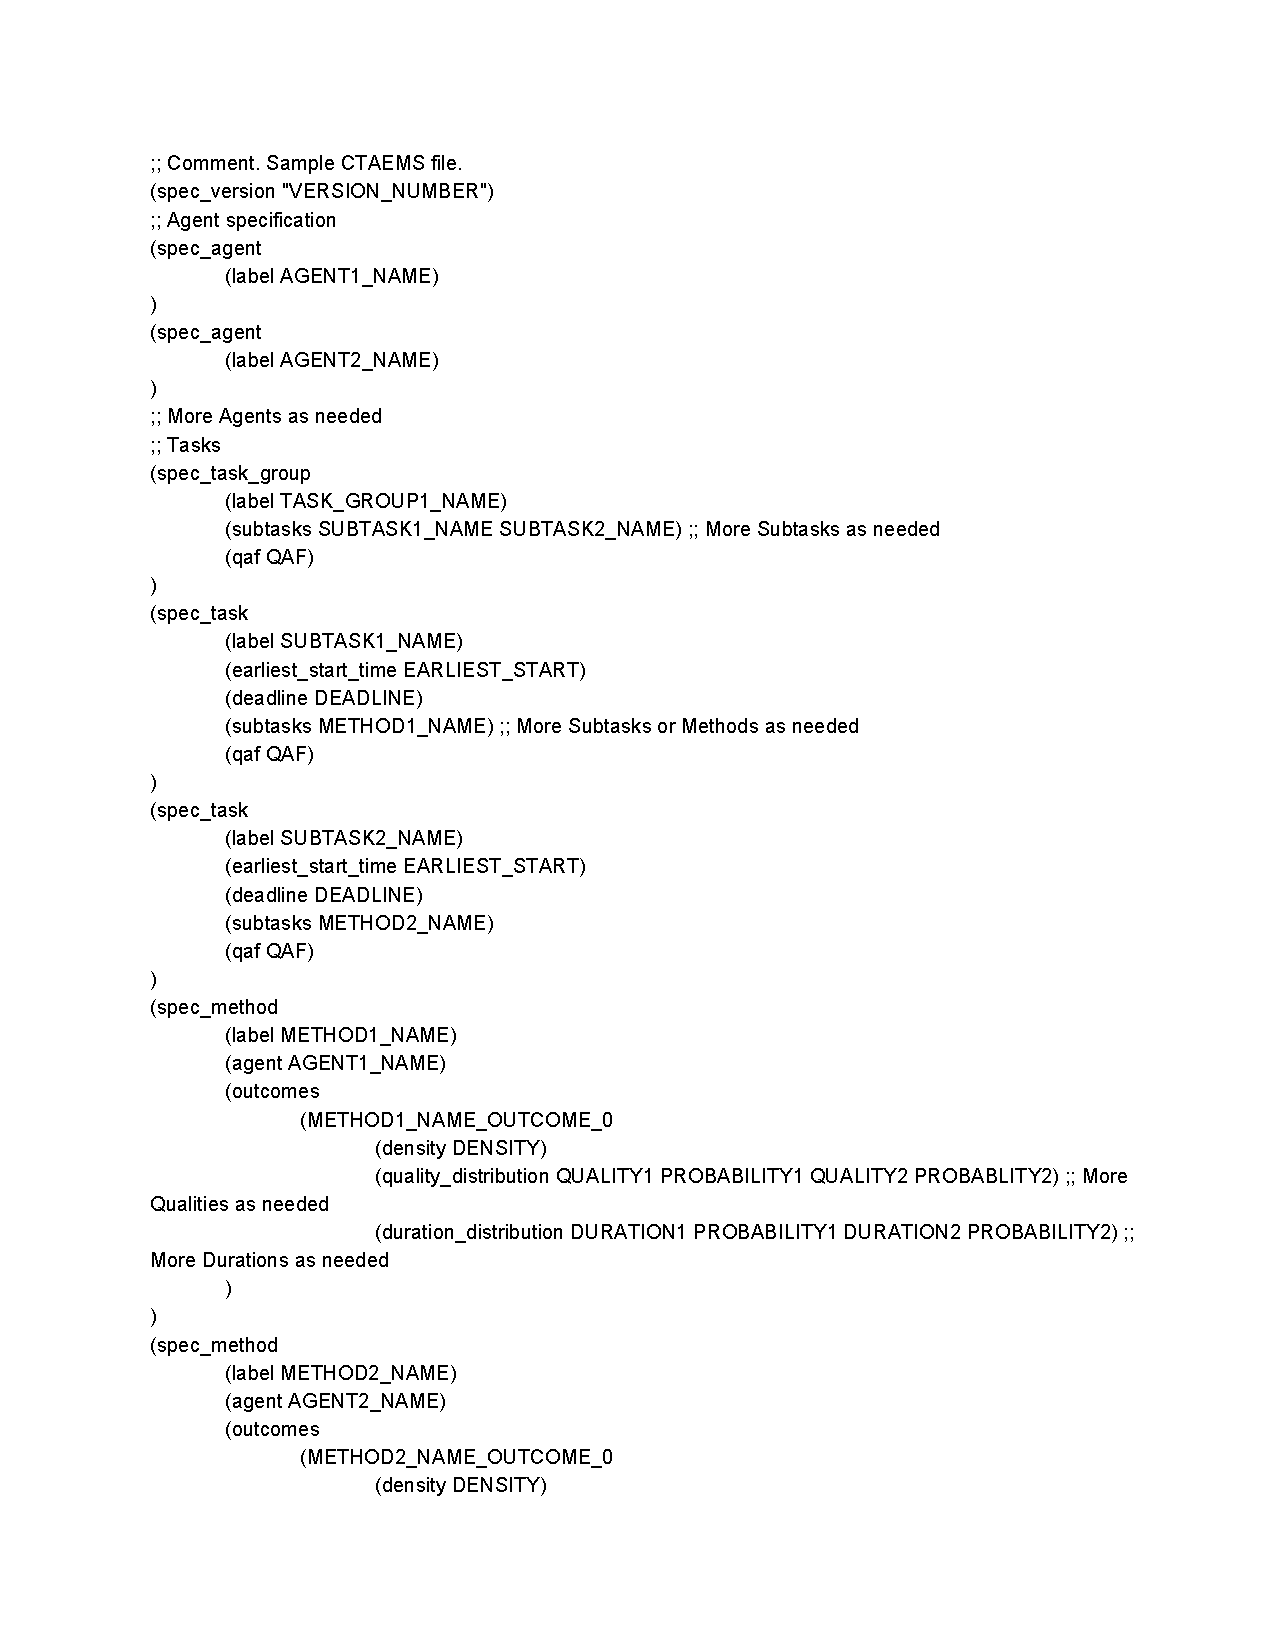
\includegraphics[page=1, width=4.6in]{figs/cTAEMS.pdf}
\caption{cTAEMS File Grammar part 1}
\label{fig:cTAEMS}
\end{figure}

\begin{figure}[H]
\centering
\includegraphics[page=2, width=4.6in]{figs/cTAEMS.pdf}
\caption{cTAEMS File Grammar part 2}
\label{fig:cTAEMS}
\end{figure}
  
  \item \textbf{Configuration File Input (CFI)}: The program by default will look for a plain text configuration file in the current directory. Optionally, a user can specify the location of this CFI.
  \begin{enumerate}
    \item If no configuration file is found the system will make one in the current directory with default values.
    \item The CFI will contain a random number seed, output file destination, the length (in milliseconds) of each Tick, and the port for the Simulator to listen on.
    \item Not all items in the CFI need to be specified. The system will resort to default values for the missing items.
    \item A sample CFI is shown in Figure 3.4.
  \end{enumerate}

\begin{figure}[H]
\centering
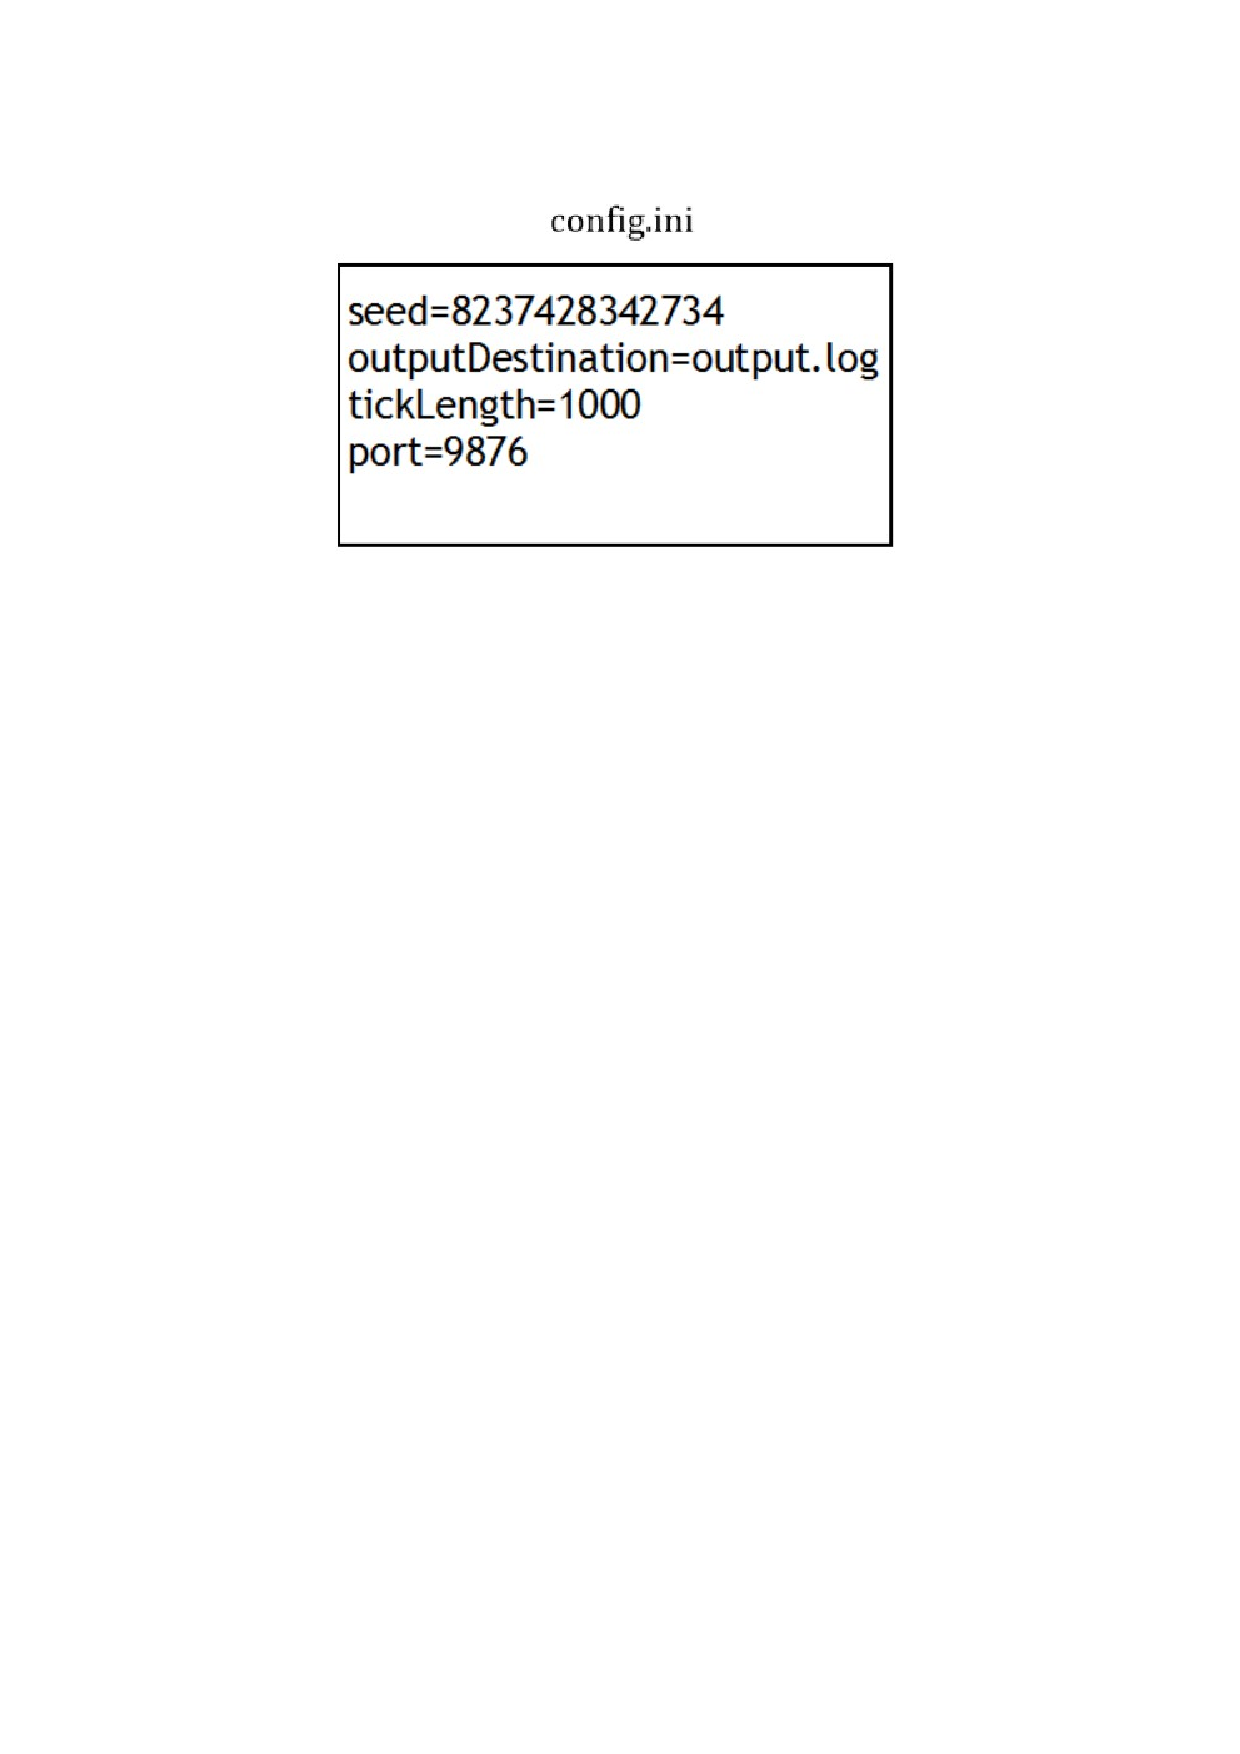
\includegraphics[width=4in]{figs/CFI.pdf}
\caption{Example CFI}
\label{fig:CFI}
\end{figure}
  
  \item\textbf{Agent Facing Interface}: The system will provide a consistent interface of which all Agents must implement in order to connect to the internal communication model.
  \begin{enumerate}
    \item All communication between the Agents and the MASS will be represented in the JSON format.
    \item The system must handle any Agent architecture in compliance with the Agent Interface (by using the correct JSON format of messages) and refuse connection to any Agent in violation of this. If an Agent does use the correct format for JSON messages, the Simulator will terminate.
    \item It is the job of the agent to choose from the available Methods and report to the Simulation when starting and event.
    \item The Simulator will tell an agent when it's Method has finished.
    \item Figures 3.5-3.13 describe the format of each Message type.
    \end{enumerate}
    
\begin{figure}[H]
\centering
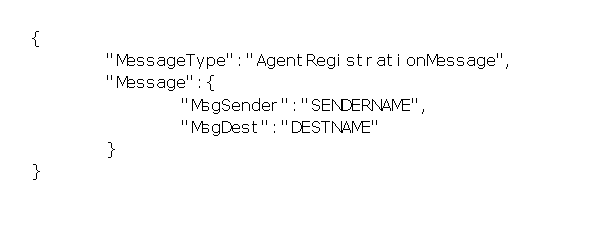
\includegraphics[width=4in]{figs/AgentRegistration.pdf}
\caption{Format of AgentRegistration Message}
\label{fig:AgentRegistration}
\end{figure}

\begin{figure}[H]
\centering
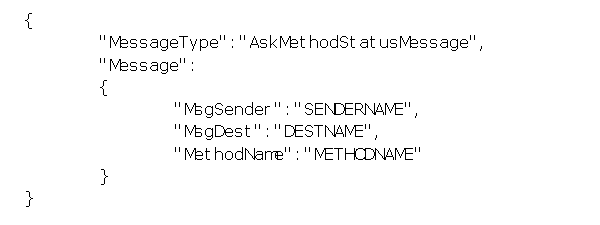
\includegraphics[width=4in]{figs/AskMethodStatus.pdf}
\caption{Format of AskMethodStatus Message}
\label{fig:AskMethodStatus}
\end{figure}

\begin{figure}[H]
\centering
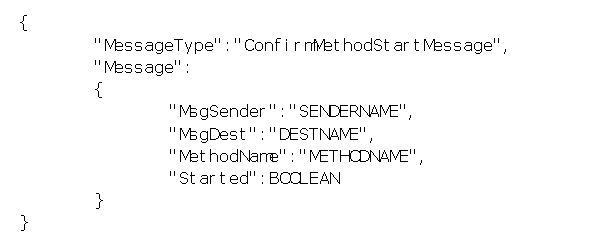
\includegraphics[width=4in]{figs/ConfirmMethodStart.pdf}
\caption{Format of ConfirmMethodStart Message}
\label{fig:ConfirmMethodStart}
\end{figure}

\begin{figure}[H]
\centering
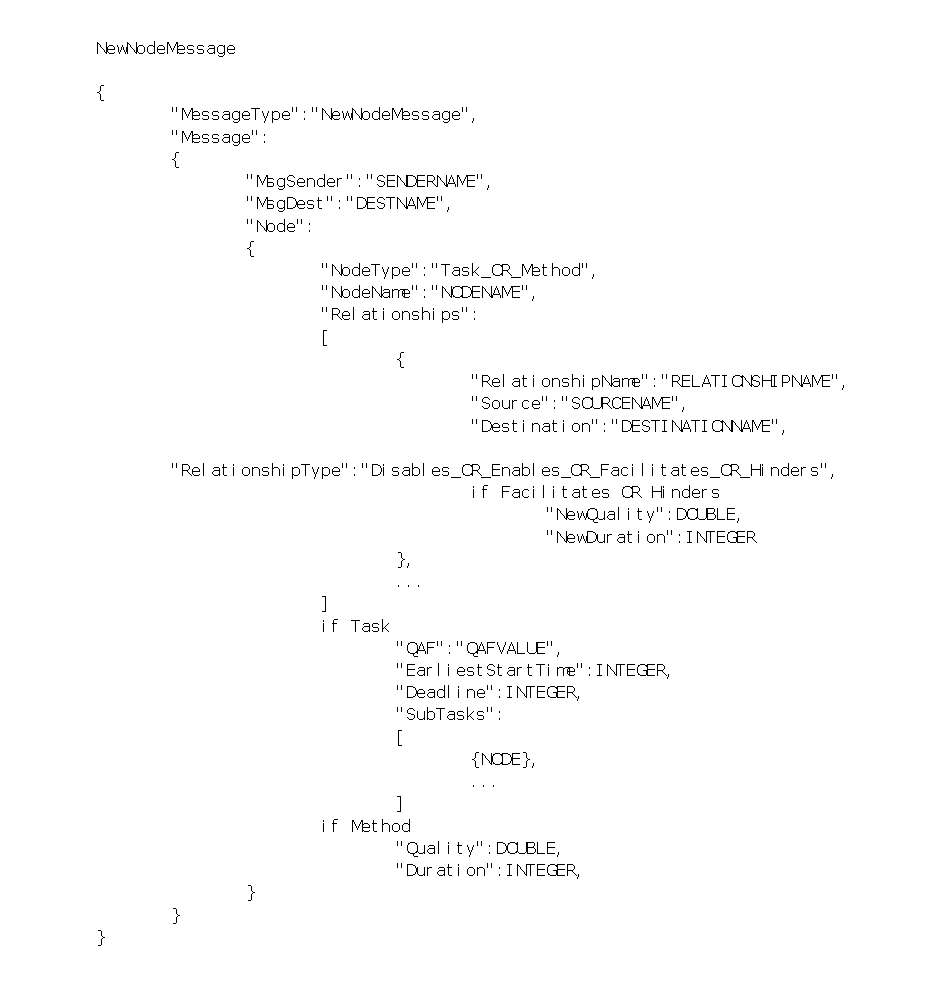
\includegraphics[width=5in]{figs/NewNodeMessage.pdf}
\caption{Format of NewNode Message}
\label{fig:NewNodeMessage}
\end{figure}

\begin{figure}[H]
\centering
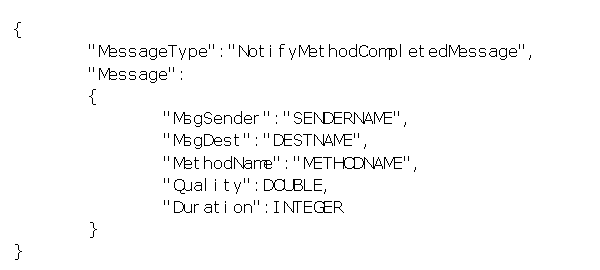
\includegraphics[width=4in]{figs/NotifyMethodCompleted.pdf}
\caption{Format of NotifyMethodCompleted Message}
\label{fig:NotifyMethodCompleted}
\end{figure}

\begin{figure}[H]
\centering
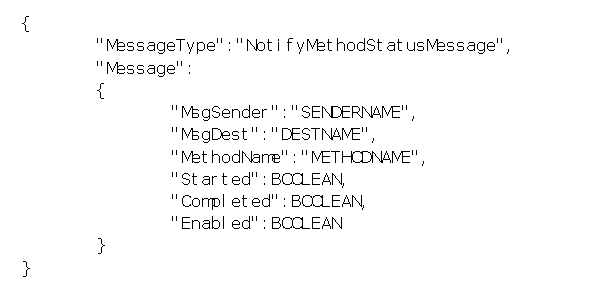
\includegraphics[width=4in]{figs/NotifyMethodStatus.pdf}
\caption{Format of NotifyMethodStatus Message}
\label{fig:NotifyMethodStatus}
\end{figure}

\begin{figure}[H]
\centering
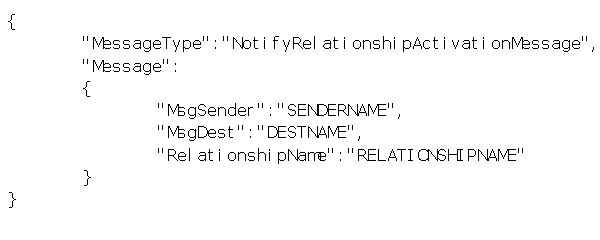
\includegraphics[width=4in]{figs/NotifyRelationshipActivation.pdf}
\caption{Format of NotifyRelationshipActivation Message}
\label{fig:NotifyRelationshipActivation}
\end{figure}

\begin{figure}[H]
\centering
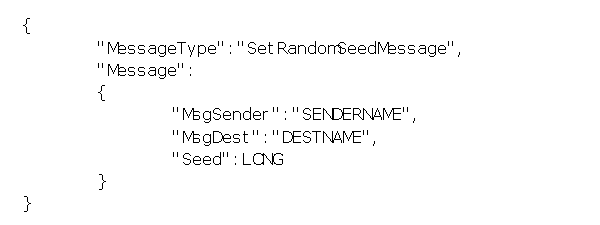
\includegraphics[width=4in]{figs/SetRandomSeed.pdf}
\caption{Format of SetRandomSeed Message}
\label{fig:SetRandomSeed}
\end{figure}

\begin{figure}[H]
\centering
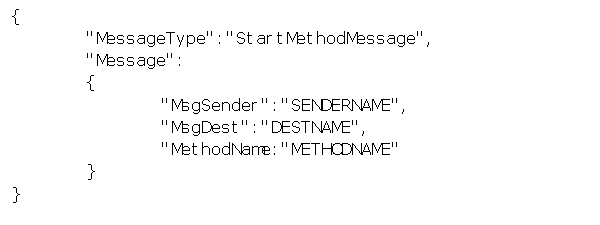
\includegraphics[width=4in]{figs/StartMethod.pdf}
\caption{Format of StartMethod Message}
\label{fig:StartMethod}
\end{figure}
    
    \item\textbf{Agent Communication}: Agents must have the ability to communicate throughout the Simulation.
    \begin{enumerate}
    \item An Agent can send a message intended for another Agent, or it can send one directly to the Simulator. Either way, the message will pass through the Simulator so that it may log the communication patterns of the Agents.
  \end{enumerate}
  
  \item\textbf{Task Tree}: A Simulation will consist of a Task Tree that keeps track of what Methods are able to be executed at any given time.
   \begin{enumerate}
    \item The Task Tree consists of Tasks and Methods. Tasks can have Nodes as children while Methods are the leaves of the tree. The total quality of a Task Group is determined from the head of that group's Task Tree.
    \item When a Method is finished, it's quality will propagate up through the tree based on its parents' QAFs.
    \item An example Task Tree showing three Tasks, four Methods, and two Relationships is shown in Figure 3.14.
  \end{enumerate}

\begin{figure}[H]
\centering
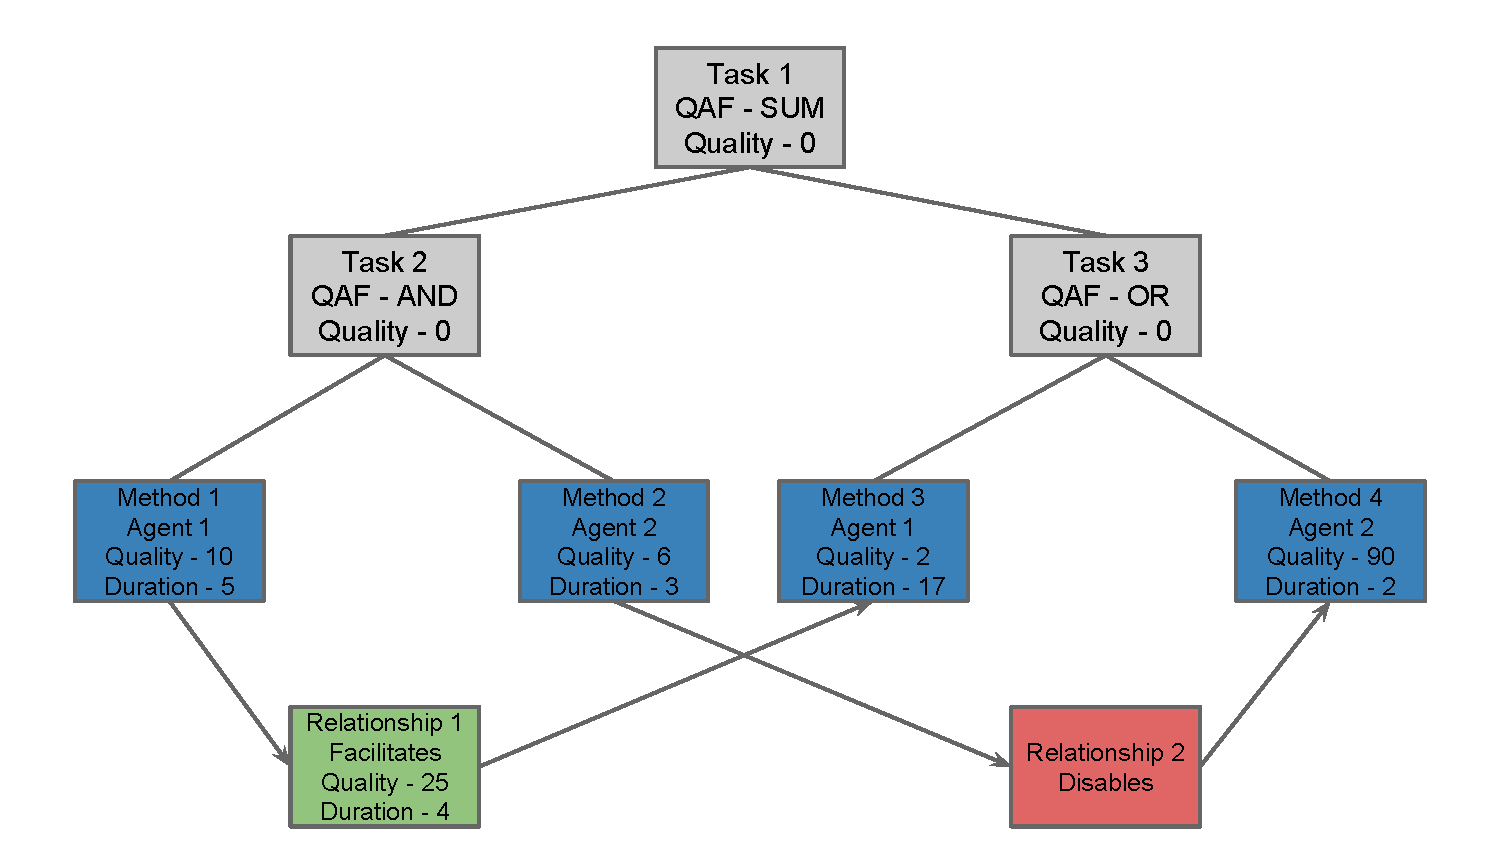
\includegraphics[width=6.5in]{figs/TaskTree.pdf}
\caption{Example Task Tree with Relationships}
\label{fig:TaskTree}
\end{figure}
  
  \item\textbf{Creating a Simulation}: A Simulation must be repeatable.
   \begin{enumerate}
    \item Any probability distributions must be computed using the seed value obtained from the CFI as the SFI is being parsed.
    \item Agents must be given the seed value obtained from the CFI in case they use any random calculations in their logic.
    \item Agents are given an initial set of Nodes that are visible to them at the start of the Simulation. Visibility is defined as follows:
    	\subitem An Agent can see its assigned Methods.
    	\subitem An Agent can see all Tasks that are direct ancestors of its Methods.
    	\subitem An Agent can see all Relationships that have one the Agent's visible Nodes as the source/target.
    	\subitem An Agent can see the Nodes that are the sources/targets of a relationship with one of that Agent's visible Relationships.
    \item When any Node or Relationship is visible to an Agent, that Agent knows:
    	\subitem The name of the Node or Relationship
    	\subitem The names of all other Agents that can see that Node
    \item When a Method is visible to an Agent, that Agent knows:
   	\subitem The Method's quality
	\subitem The Method's duration
    \item When a Task is visible to an Agent, that Agent knows:
   	\subitem The Task's QAF
   	\subitem The Task's (visible) Subtasks
    \item When a Relationship is visible to an Agent, that Agent knows:
    	\subitem The type of the Relationship
    	\subitem The source and target of the Relationship
    	\subitem The new quality and duration if the Relationship is of Facilitates or Hinders type
  \end{enumerate}
  
  \item\textbf{Running a Simulation}: The MASS must keep track of Nodes.
    \begin{enumerate}
    \item The MASS must know what Methods are able to be executed at any given time.
    \item The MASS must know what Methods are being executed at any given time.
    \item The MASS must know what Methods have been executed at any given time.
    \item The MASS must know what the Qualities of all Tasks are at any given time.
    \item The MASS must know which Tasks have been completed at any given time.
    \item The MASS must know when the Simulation is finished. This is achieved when every Task Group has no Methods that are both enabled and unfinished.
  \end{enumerate}
  
  \item\textbf{Simulation Output}: The system will produce an output detailing the overall Quality and Duration of the entire Simulation.
  \begin{enumerate}
  \item The output should occur on the command line.
  \end{enumerate}
  
  \item\textbf{Log File Output (LFO)}: The system will produce a detailed log file including the intermediate Quality and Cost between every Task and Method.
  \begin{enumerate}
  \item The LFO will contain a transcript of Agent communication
  \item The LFO will contain compiled statistics on Agent communication frequency.
  \item The LFO will contain the intermediate and final Quality, Cost, and Duration that results from completing an Event in the Task Tree.
  \end{enumerate}

\end{enumerate}


\begin{center} \textbf{Additional Features} \end{center}

\begin{enumerate}

\item\textbf{Graphical Representation of Task Tree}:  The Task Tree is a hierarchical tree-like structure representing Nodes and the Relationships between them.
\begin{enumerate}
\item The system may represent this structure as a graphical model to help understand the Simulation results better. 
\end{enumerate}

\item\textbf{cTAEMS Grammar Support}: The system may go beyond the logical AND, OR, and SUM operations and include additional implementations within the cTAEMS grammar.

\item\textbf{Agent Behavior}: The System may support the ability of Agents to stop, pause, or resume Methods if such actions are applicable based on the Simulation specifications. 

\end{enumerate}

\chapter{Other non-functional requirements}\label{chapter:otherFunctionalRequirements}

\section{Performance requirements}

All Agents involved with the model are connected to the simulator using sockets. The Agents themselves are independent processes, which could run on physically different machines. Note that the simulator does not control the Agents' activities, it merely allocates time slices and records the Events performed by the Agent during the time slice. This makes the performance of the MASS independent of an Agents performance. The system shall function in real-time, however, the effect of network load or maximum limit on socket connections can only be published after testing.

\section{Maintainability}

The standardized design and implementation documents will be provided in order to maintain the system. All changes will be documented. A standard architecture will be applied and therefore allowing for quick evolution of the software to adapt to possible situations in the future. 

\section{Software Quality Attributes}

The user interface of the Multi-Agent System Simulator is to be designed with usability as the first priority. The system will be presented and organized in a manner that is both visually appealing and easy for the user to navigate. To ensure reliability and correctness, there will be zero tolerance for errors in the Simulation environment. 



% !TEX root =  thesis.tex
\chapter{Detailed System Description}\label{detailedSystemDescription}

\section{Design overview}

The system is broken into five major packages called application, input, output, simulation, and tasktree. Figure 5.1 shows the relationship between these components.

\begin{figure}[H]
\centering
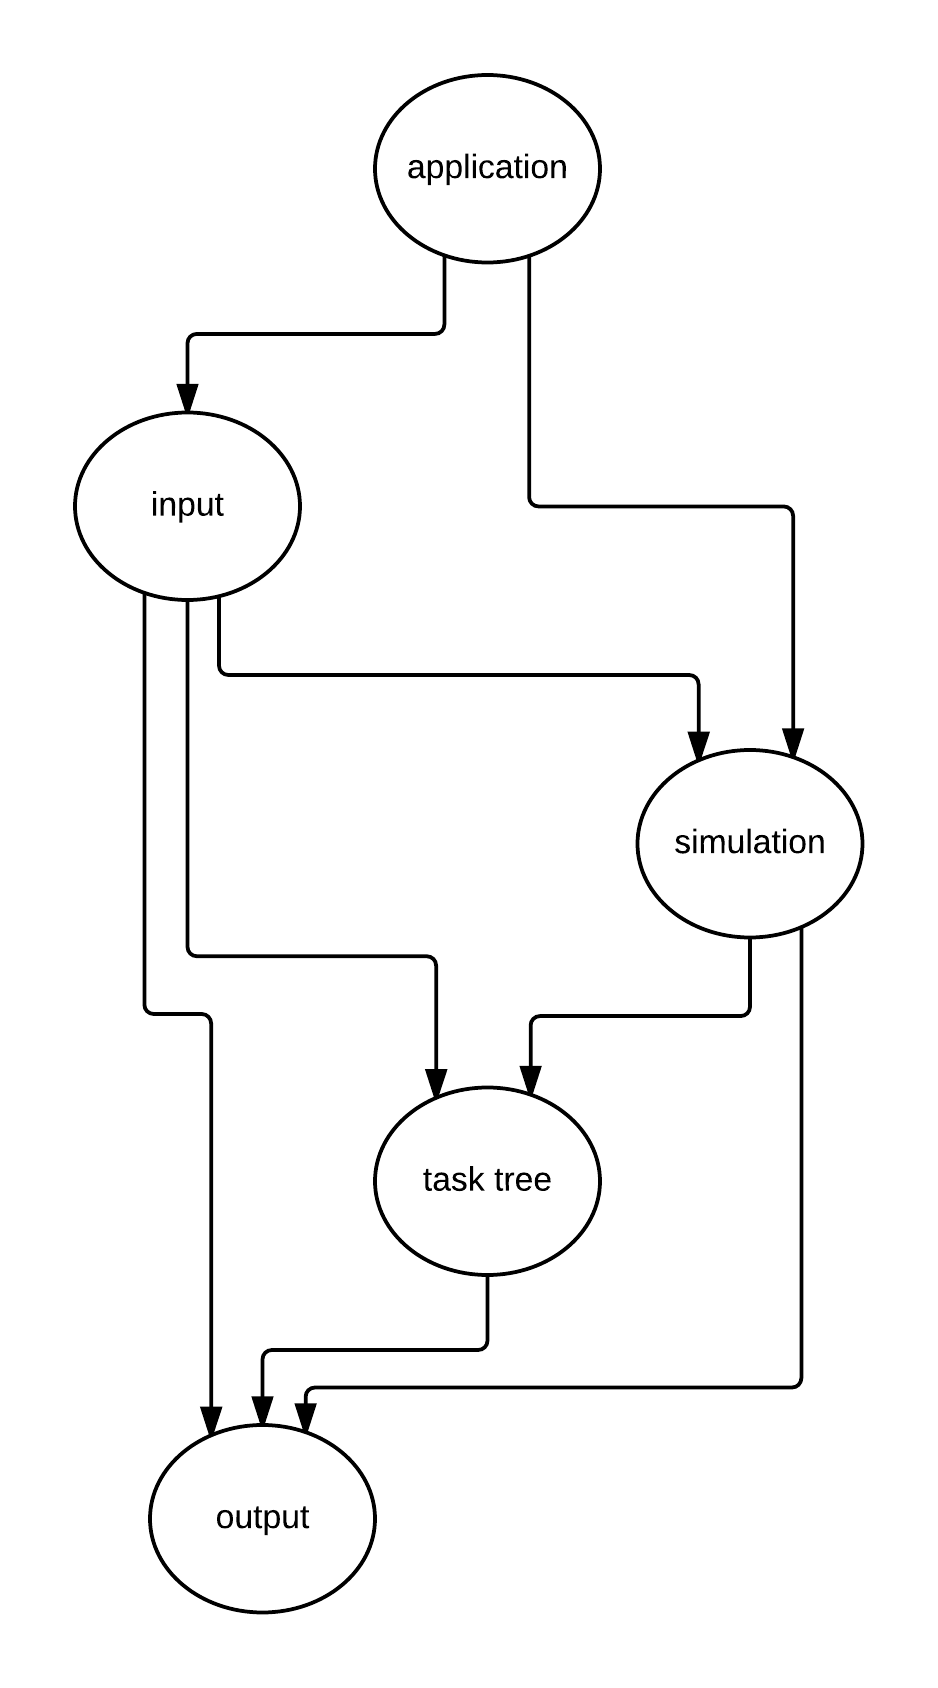
\includegraphics[trim=0.5cm 4.0cm 0.5cm 0.5cm,width=4.0in]{figs/UsesDiagram}
\caption{USES diagram for packages within MASS.}
\label{fig:UsesDiagram }
\end{figure}

\section{Package Overview}

\begin{enumerate}

\item\textbf{application}
\begin{itemize}
\item Description: The application package is responsible for initializing the other packages and linking everything together.
\item Contains: The application package contains module AISim.
\item Uses: This package uses the input, and simulation packages.
\end{itemize}

\item\textbf{input}
\begin{itemize}
\item Description: The input package is responsible for reading the initial data input and building a Task Tree to represent this data.
\item Contains: The input package contains three modules which include Parser, ConfigurationData, and InputData.
\item Uses: This package uses the tasktree, and simulation packages.
\end{itemize}

\item\textbf{simulation}
\begin{itemize}
\item Description : The simulation package is responsible for connecting and communicating with agents, managing the Task Tree, and advancing the clock. Figure 5.2 represents the USES diagram for the package simulation.
\item Contains : This package contains the modules Simulator, Agent, Message and ServerThread.
\item Uses : This package uses the tasktree and output packages.
\end{itemize}

\item\textbf{tasktree}
\begin{itemize}
\item Description : The tasktree package is responsible for representing the Task Tree in a hierarchical manner that is easy for the simulation package to update and distribute.
\item Contains : This package contains the modules Node, NodeRelationship, and Distribution.
\item Uses : This package does not use any packages.
\end{itemize}

\item\textbf{output}
\begin{itemize}
\item Description: The output package is responsible for printing data after the simulation has completed. It is also responsible for logging detailed data to a file during the course of the simulation.
\item Contains: The output package contains a module Logger.
\item Uses: This package does not use any packages.
\end{itemize}

\begin{figure}[H]
\centering
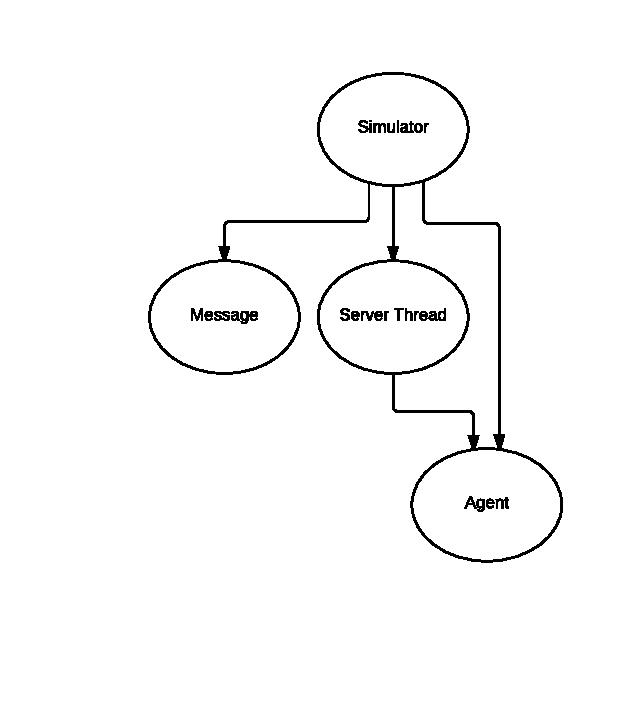
\includegraphics[trim=0.5cm 2.5cm 0.5cm 1.0cm, width=3.5in]{figs/simPackage}
\caption{Uses diagram for the package simulation}
\label{fig:simulation}
\end{figure}

\end{enumerate}

\section{Detailed Package Design}

\begin{enumerate}

\item \textbf{Application}  The application package is responsible for initializing the modules within the input and simulation packages in order to begin the Simulation.

\begin{figure}[H]
\centering
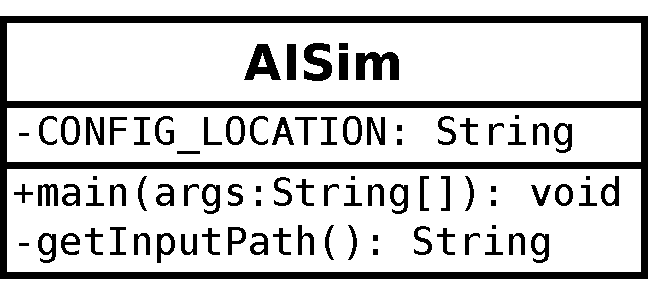
\includegraphics[width=1.5in]{figs/applicationUML}
\caption{UML diagram for input package}
\label{fig:input}
\end{figure}

\item \textbf{Input} Figure 5.3 represents the UML class diagram for input package. This package is responsible for reading and parsing the cTAEMS SFI and the plain text CFI. This packages contains an abstract parser which serves as a template for the InputParser and the ConfigurationParser. \\

\begin{itemize}
\item \textbf{InputParser}: The InputParser is responsible for reading the SFI which contains definitions for Agents, Nodes, and Relationships that make up the Simulation. The first step of the parse involves reading the desired cTAEMS file into a string by implementing Java's BufferedReader class. Second, the string is split into tokens such as Agent, Task, Task Group, Method, and Relationship. These tokens are further parsed in order to analyse their various components. For example, a Task could be broken up into a label, list of Subtasks and QAF which are instantiated into the corresponding Task class. This data is used to build an instance of the TaskTree class which is then stored in the InputData class which will be passed to the simulation. \\

\begin{figure}[H]
\centering
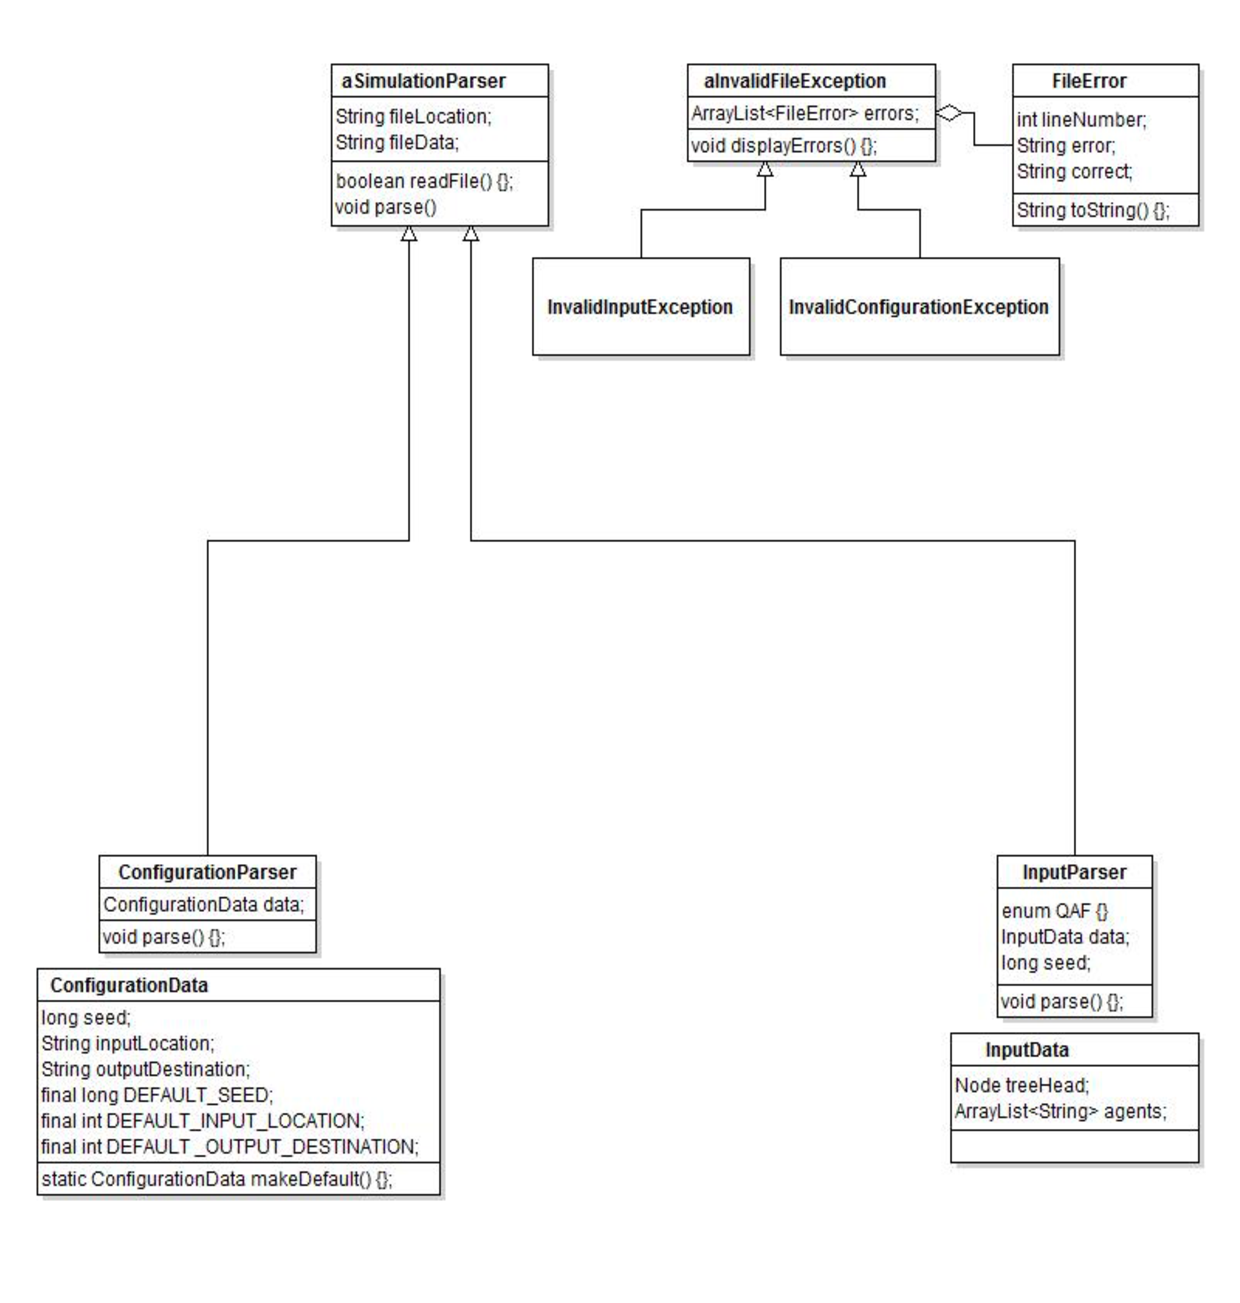
\includegraphics[width=5.0in]{figs/inputUML}
\caption{UML diagram for input package}
\label{fig:input}
\end{figure}


\item \textbf{ConfigurationParser}: The configuration parser reads and parses the CFI to determine the random seed used throughout the Simulation. The Configuration parser will use Java's BufferedReader class to read in the file, with the first line representing the seed, the second the input location, the third output destination, the fourth the length of a tick, and finally the communication port. This data is written to the ConfigurationData class which is sent to the simulator. \\

\item \textbf{Exceptions}: Within the input package there are three exceptions which are used to report a problem encountered during a parse. These exceptions are: InvalidFileException, InvalidInputException, and InvalidConfigurationException. InvalidInput and InvalidConfiguration both inherit from InavlidFile. \\
\end{itemize}

\begin{figure}[H]
\centering
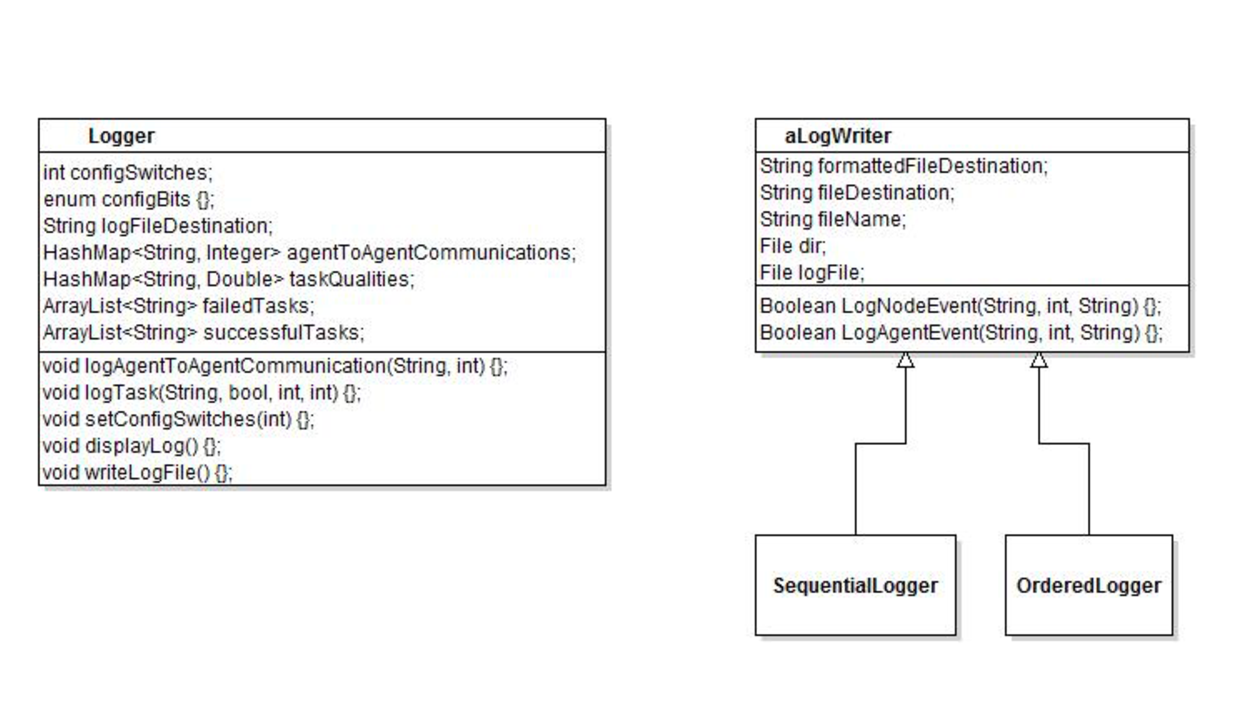
\includegraphics[width=2.0in]{figs/outputUML}
\caption{UML diagram for output package}
\label{fig:output}
\end{figure}

\item \textbf{Output} Figure 5.4 represents the UML diagram for output package. The output package is responsible for logging data after the simulation has completed. It contains a Logger class which upon completion will create the LFO document. \\

\begin{itemize}
\item \textbf{Logger}: The Logger class is responsible for producing a  transcript of Agent communication, statistics on Agent communication frequency, and the intermediate and final Quality and Duration that results from completing a Node in the Task Tree. Data will be passed to the Logger by the modules within the simulation package as the simulation advances. Upon completion of a simulation, the Logger will compile statistics on agent communication and produce the LFO containing the previously mentioned data. \\
\end{itemize}

\item \textbf{Simulation}  Figure 5.5 represents the UML diagram for simulation package. The simulation package is responsible for handling all of the communications with Agents as well as updating the Task Tree architecture to model the current state of the simulation. \\

\begin{itemize}
\item \textbf{Simulator}: This class contains all of the information about the simulation such as the random number seed, the Task Tree instance, the list of currently connected Agents, the Logger object, the list of currently running Methods, and the ServerCommunicateThread. This class is the core timekeeper of the simulation. \\

\begin{figure}[H]
\centering
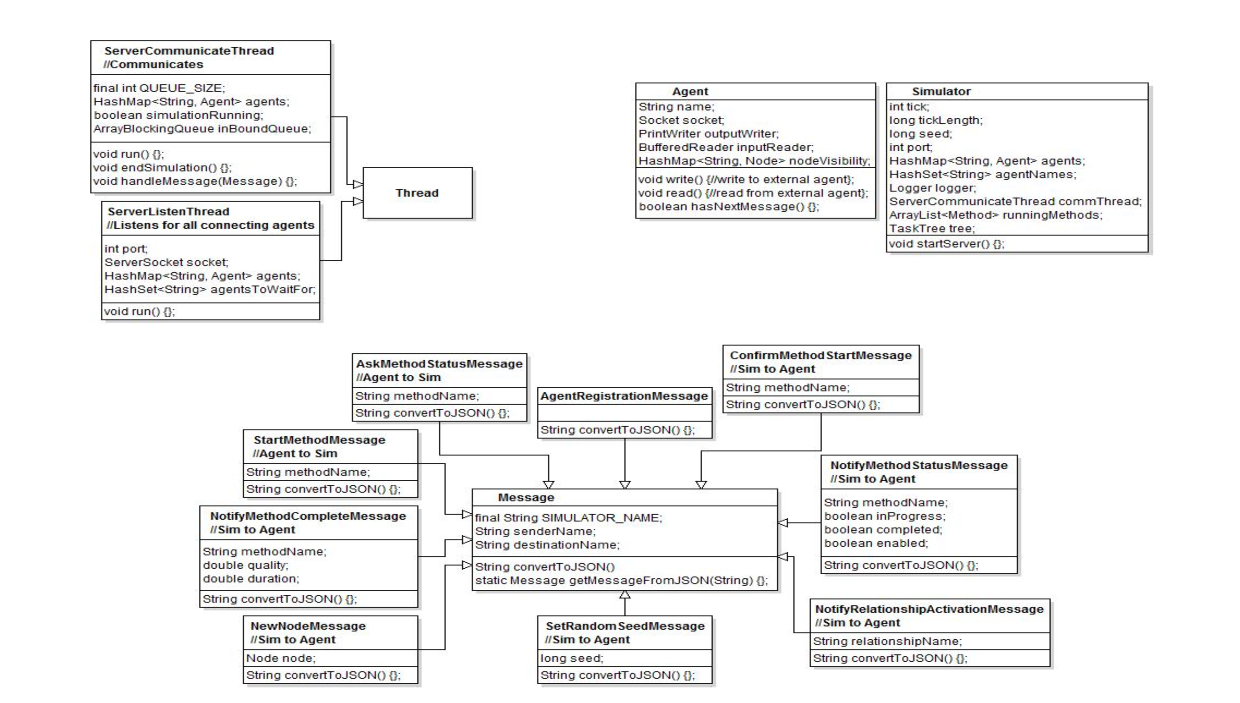
\includegraphics[width=6.0in]{figs/simulationUML}
\caption{UML diagram for Simulation package}
\label{fig:Simulation}
\end{figure}



\item \textbf{Agent}: This class is used to encapsulate all the relevant information about an Agent such as its name, and HashMap of visible Nodes. This class also contains a PrintWriter and BufferedReader that are used to communicate with the external Agent program that it represents. \\

\item \textbf{ServerListenThread}: This Thread will listen for new Agents that are trying to connect to the simulation. If an Agent connects with a valid name then this thread packages the Agent's information into an Agent object so that it can be accessed and communicated with throughout the simulation. \\

\item \textbf{ServerCommunicateThread}: This Thread will create and process all Messages coming in from and going out to all Agents in the simulation. It contains a queue of received messages that the Simulator will dump and process at the start of each tick.\\

\item \textbf{Message}: This class contains the base information for a Message such as the senderName, and the destinationName. There are many subtypes of Messages listed below. It also has a factory method to allow the creation of a new Message from a received JSON string.\\

\subitem \textbf{(i) StartMethodMessage}: Tells the Simulator that the Agent wants to start a Method.
\subitem \textbf{(ii) ConfirmMethodStartMessage}: Tells an Agent that they have successfully started a Method. 
\subitem \textbf{(iii) AskMethodStatusMessage}: Ask the Simulator for the status of a currently running Method.
\subitem \textbf{(iv) NotifyMethodStatusMessage}: Tells an Agent the status of a currently running Method.
\subitem \textbf{(v) NotifyMethodCompleteMessage}: Tells an Agent that their Method has completed and what the result is.
\subitem \textbf{(vi) NewNodeMessage}: The Simulator tells the Agent about it's initial visible nodes.
\subitem \textbf{(vii) SetRandomSeedMessage}: Tells an Agent to set their random number seed to a specified number.
\subitem \textbf{(viii) NotifyRelationshipActivationMessage}: Tells an Agent that a NodeRelationship was activated and what the result is.
\subitem \textbf{(ix) AgentRegistrationMessage}: Ask the Simulator to register this Agent into Simulation.\\
\end{itemize}

\begin{figure}[H]
\centering
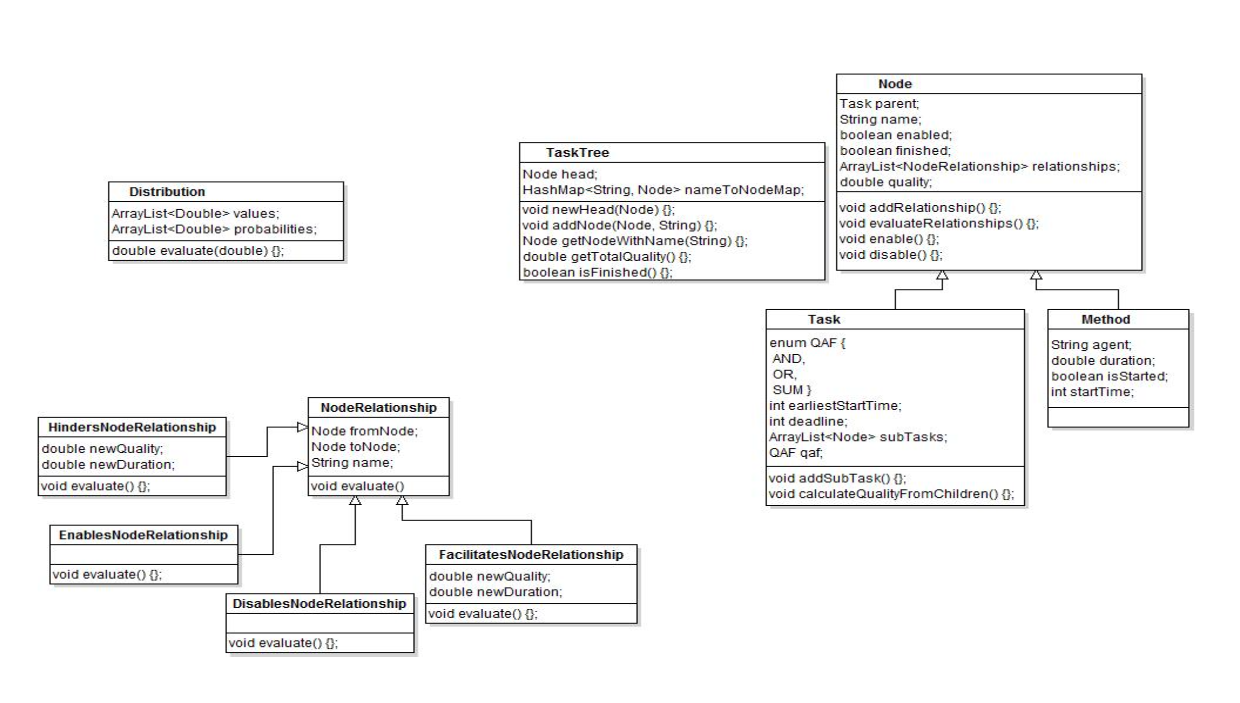
\includegraphics[width=6.0in]{figs/tasktreeUML}
\caption{UML diagram for tasktree package}
\label{fig:TaskTreeUML}
\end{figure}

\item \textbf{Tasktree} This package provides a framework for building a Task Tree. It is used by the input package to construct a programmatic representation of the SFI including Task, Methods, and Node relations. \\

\begin{itemize}

\item \textbf{TaskTree}: A wrapper class for the whole Task Tree. Contains a reference to the head Node of the tree. Also contains some methods to allow easily information gathering about the tree.

\item \textbf{Node}: The base Node class that contains all the information about a Node of the tasktree such as Quality, name, this Nodes parent Node, a list of NodeRelationships from this Node, whether or not the Node is enabled, and whether or not the Node is finished. \\

\item \textbf{Task}: A Task is a type of Node whose completion is defined by its Subtasks. A Task's completion quality is the result of it's QAF being run. More Quality options can be added as needed. A Subtask can either be another Task which would have more Subtasks or a Method which has no Subtasks. \\

\item \textbf{Method}: A Method is a Node that can be completed by a specific Agent. The Method contains a Duration which is the amount of time it takes to complete the Method. Methods can have their Duration and Quality modified by the FacilitatesNodeRelationship and HindersNodeRelationship. \\

\item \textbf{NodeRelationships}: There are many NodeRelationships that represent the affect that the completion of one Node has on another. The types of NodeRelations are below. \\

\subitem \textbf{(i) HindersNodeRelationship}: Completing one Node decreases the Quality and increases the Duration of a Method.

\subitem \textbf{(ii) FacilitatesNodeRelationhip}: Completing one Node increases the Quality and decreases the Duration of a Method.

\subitem \textbf{(iii) EnablesNodeRelationship}: The completion of the first Node enables the starting of the second Node

\subitem \textbf{(iv) DisablesNodeRelationship}: The completion of the first Node disables the starting of the second Node.

\item \textbf{Distribution}  A Distribution is used to generate Qualities and Durations for the Nodes. It is given a probability distribution specified in the cTAEMS file and a random number. The Distribution then calculates which value it should return.


\end{itemize}
\end{enumerate}
\chapter{Verification Plan}\label{verification}

\section{Verification Plan}

The verification plan and testing is the process of evaluating a system or component during or at the end of the development process to determine whether it satisfies specified requirements. We write a test prior to implementing a requirement in order to cover the requirement. Post implementation of the requirement we write additional tests to cover any statements which were not covered by the previous tests. The testing strategy for the Multi-Agent System Simulator is a combination between black box and white box testing.

\begin{enumerate}

\item \textbf{Black Box Testing:} The objective of black-box testing is to verify the functionality of the Simulator. Here, each module is treated as a 'black-box', whose internals cannot be seen. We examine the specification of each module by defining different
input scenarios that would result in different behaviour. We use the input and the output packages and perform tests to verify the desired output and the state of the simulator.

\item \textbf{White Box Testing:} For the purpose of white box testing we will be making use of test coverage tools to measure the statement coverage, branch coverage and missed lines. Each module and subsequent files related to the module will generate these statistics. We test the application module, input module, simulation module, task tree module and the output module which forms the overall structure of the Multi-Agent System Simulator. For each of these modules we aim at achieving 95-100% coverage, the fact that the simulation package generates threads, each time we test the class generates the thread which is not in the scope of Unit tests. This can be tackled if we employ an integration test strategy.

\begin{itemize}
\item \textbf{Unit Testing:} Unit tests are performed during the implementation process on individual units of the source code. For unit testing, all the test cases shall be implemented using the JUnit Test Suite. For each test case, there shall be an expected output and an actual output. If the actual output matches the expected output, the test case shall pass; otherwise, it shall fail. In table 6.1 and 6.2 we represent all the tests performed so far.

\begin{table}[H]

\caption{Test Status Report} % title of Table 
\begin{tabular}{| l | p{4cm} | p{4cm} | p{4cm} | l |} 
\hline\hline %inserts double horizontal lines 
 Test ID & Test Class & Test Name &  Description & Status \\ [0.5ex] % inserts table 
%heading  
\hline % inserts single horizontal line 
T1 & ConfigurationDataTest & testMakeDefault, basicConstructorTest & Tests the configuration file data and generation of a default configuration file. & Success \\ % inserting body of the table 
T2  & ConfigurationParserTe- \ st & testParse & Test if the data is parsed in accordance to the ConfigurationParser &  Success \\ % inserting body of the table  \\
T3 & FileErrorTest & testToSpring, testFileError, testExceptions & Test for correctness for the input file. &  Success \\ % inserting body of the table \\
T4 & FileExceptionsTest & testExceptions & Test the input and configuration files for handling exceptions. &  Success \\
T5 & InputParserTest & basicConstructorTest, testParse, exceptionTest, testNotNull & Test for valid input data and exception handling &  Error \\
T6 & OrderedLoggerTest & testformattFileDest- \ inationOne & Test the log events for all tasks and methods &  Success \\
T7 & SequentialLoggerTest & testformattFileDest- \ inationOne, testformattFileDestinationOne & Test the format of the generated logger file. &  Success \\
T8 & AgentRegistrationMes- \ sageTest & toJSONTest &  If the AgentRegistrationMessage is in accordance with JSON structure. &  Success \\
T9 & AskMethodStatusMess- \ ageTest &  toJSONTest & If the AskMethodStatusMessage is in accordance with JSON structure. &  Success \\
T10 & ConfirmMethodStart- \ MessageTest & toJSONTest & Checks status for start method message. &  Success \\

T11 & MessageTest & getMessageFromJSON- \ UnknownTest, getMessageFromJSONTest & Test for all message exchanges. &  Success \\
\hline %inserts single line  \\
\end{tabular} 
\label{table:nonlin} % is used to refer this table in the text 
\end{table} 

\begin{table}[H] 
\caption{Test Status Report} % title of Table 
\begin{tabular}{| l | p{4cm} | p{4cm} | p{4cm} | l |} % centered columns (4 columns) 
\hline\hline %inserts double horizontal lines 
 Test ID & Test Class &Test Name &  Description & Status \\ [0.5ex] % inserts table 
%heading  
\hline % inserts single horizontal line 
T12 & NextTickMessageTest & toJSONTest & Returns the status for method NextTickMessage & Success \\
T13 & NotifyMethodCompl- \ etedMessageTest & toJSONTest & Returns the status for method on competition. &  Success \\
T14 & NotifyMethodStatusMe- \ ssageTest & toJSONTest & Returns the method status. &  Success \\
T15 & NotifyRelationshipAct- \ ivationMessageTest & toJSONTest & Returns the relationship and the sender. &  Success \\
T16 & ServerCommunicateTh- \ readTest & testRun, testHandleMessage, testBadHandleMessage, tesBadRun  toJSONTest & Check if messages are passsed from server to agent using sockets. &  Success \\
T17 & ServerListenThr- \ eadTest & testBadRunSocketFail, testBadRunCreateFail, testBadRunNullName, testBadRunReadFail, testBadRunAcceptFail & Check if messages are passed from agents to server using sockets. &  Success \\
T18 & SetRandomSeedMessa- \ geTest & toJSONTest & Test the message communication for random seed. &  Success \\
T19 & StartMethodMessageT- \ est &  toJSONTest & Checks if method initializes &  Success \\ 
T20 & AgentTest & testAgentName, testTaskTree, testSocket & Test the socket connection and the new messages from the generated task tree. &  Success \\
T21 & SimulatorTest &  testSimOneAgent, testSimFinishesTreeDone, testAgentDoMethod & Test the message exchanges in simulator for multiple agents for given input data. &  Success \\
T22 & DisablesNodeRelation- \ shipTest & testEvaluate &  Tests for the node relationship for methods. &  Success \\
T23 & DistributionTest & testEvaluate & Test to generate quality and duration for nodes.  &  Success \\
\hline %inserts single line  \\
\end{tabular} 
\label{table:nonlin} % is used to refer this table in the text 
\end{table}

\begin{table}[H] 
\caption{Test Status Report} % title of Table 
\begin{tabular}{| l | p{4cm} | p{4cm} | p{4cm} | l |} % centered columns (4 columns) 
\hline\hline %inserts double horizontal lines 
 Test ID & Test Class &Test Name &  Description & Status \\ [0.5ex] % inserts table 
%heading  
\hline % inserts single horizontal line
T24 & EnablesNodeRelation- \ shipTest &  testEvaluate & Test enables relationship for nodes. &  Success \\
T25 & FacilitatesNodeRelatio- \ nshipTest & testEvaluate & Tests facilitates relationship for nodes. &  Success \\
T26 & HindersNodeRelations- \ hipTest & testEvaluate & Tests hinders relationship for nodes. &  Success \\
T27 & MethodTest & testMethodGetSet & Tests if method returns all the attributes. &  Success \\
T28 & TaskTest & testCalculateQualityFr- \ omChildren, testCheckIsFinished, testSetQAF & Tests task tree status for a given set of tasks. &  Success \\
T29 & TaskTreeTest &  testActivateAllRelatio- \ nships, testGetTotalQuality, testGetTotalQuality, testAddNode, testComputeEarliestStartAndDeadline, testTaskTree, testFindVisibleToAgents, testNewHead, testIsFinished & Tests generation of task tree and nodes based on the input task and methods.  &  Success \\ 
T30 & InputDataTest & basicConstructorTest &  & Success \\
T31 & EndSimulationMessag- \ eTest & toJSONTest &  Checks method return message (endSimulationMessage)  & Success \\
T32 & InitialTreeMessageTest & testToJSON & Checks the return value for a given task using the task tree & Success \\ 
T33 & StartSimulationMessa- \ geTest &  toJSONTest & Checks if method initializes and returns message StartSimulationMessage &  Success \\  
\hline %inserts single line  \\
\end{tabular} 
\label{table:nonlin} % is used to refer this table in the text 
\end{table}

\item \textbf{Integration Testing:}  In this testing strategy we aim at testing combined parts of the application to determine if they function correctly together. We use a Bottom-up Integration approach where we first perform unit testing, followed by tests of progressively higher-level combinations of modules. Figure 6.1 shows the component modules that form the MASS application.
 In order to decide the number of integration tests we consider the following two criterion's: Check that all data exchanged across an interface agrees with the data structure specifications and confirm that all the control flows have been implemented.


\begin{figure}[H]
\centering
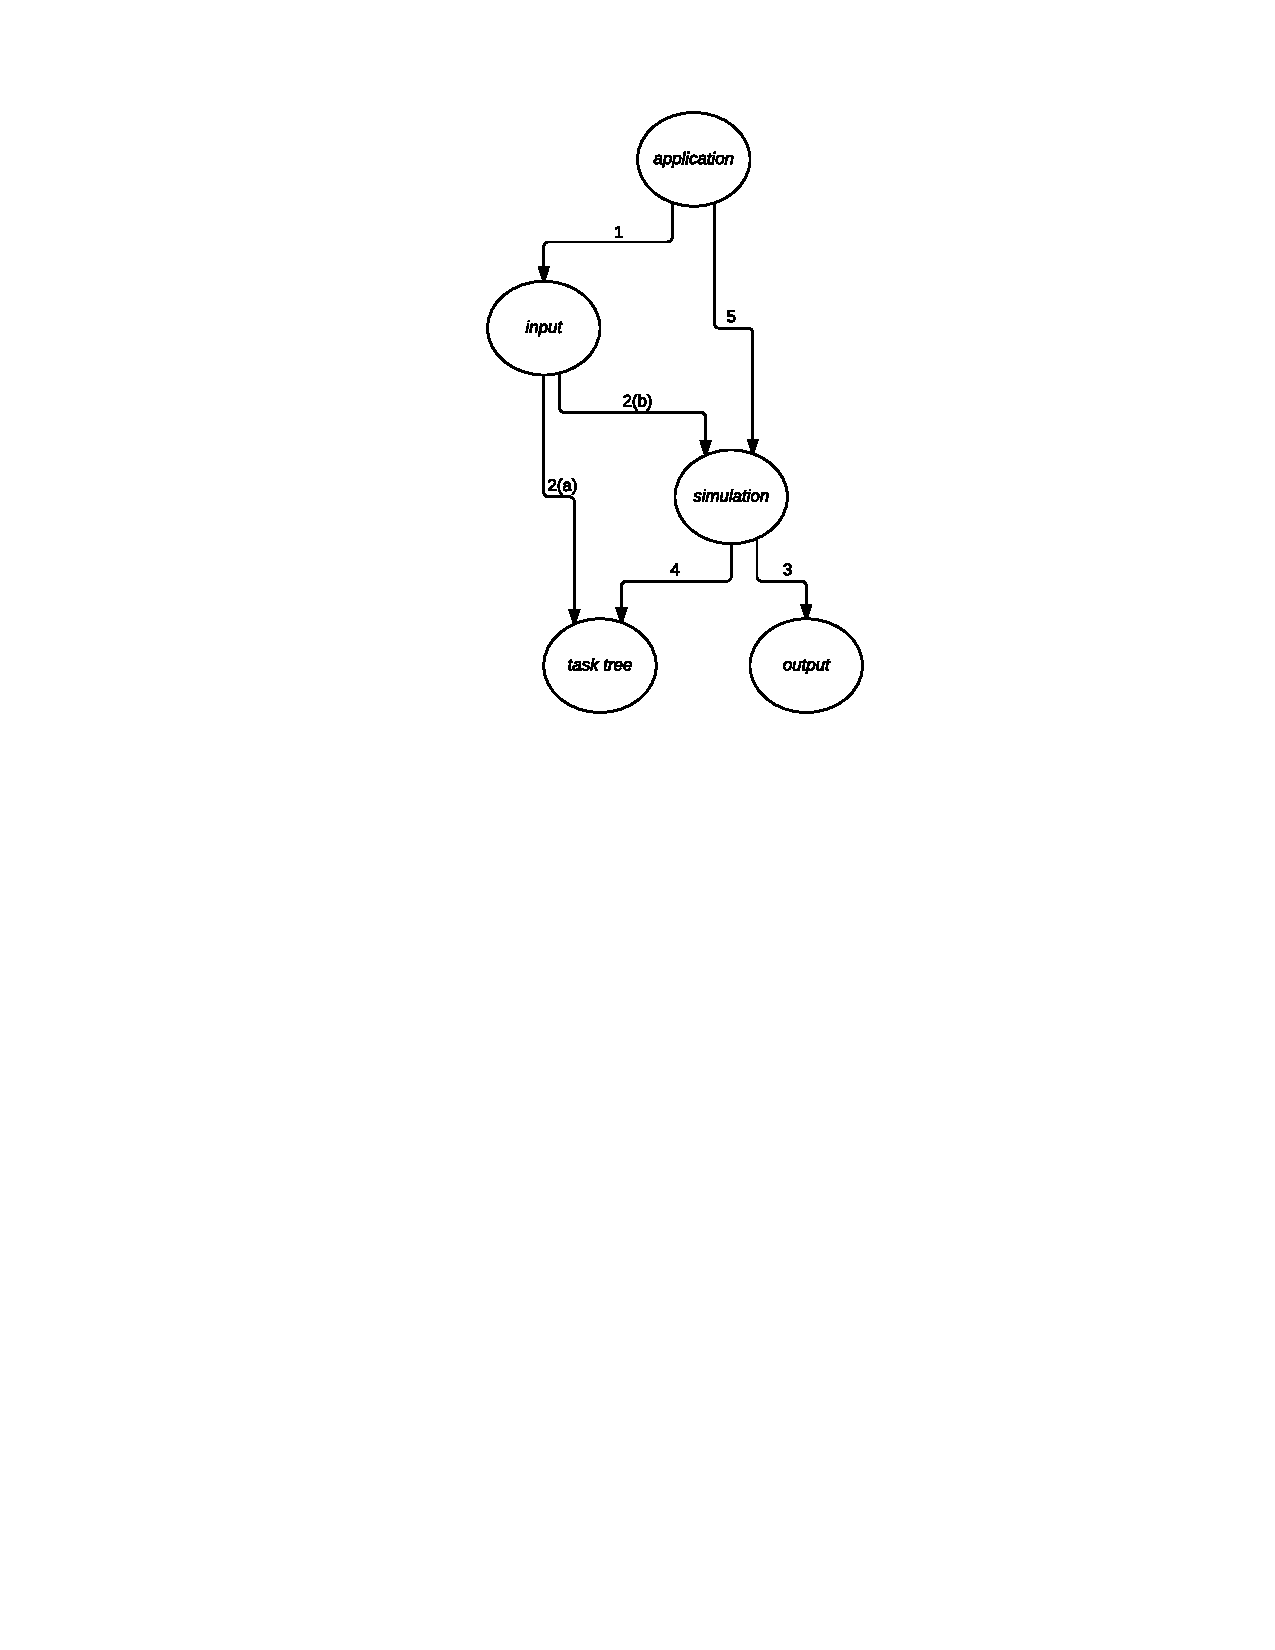
\includegraphics[trim=3.5cm 15.5cm 0cm 0cm, width=8.0in]{figs/OverviewUsesDiagram}
\caption{Overview of the USES diagram for packages within MASS.}
\label{fig:OverviewUsesDiagram }
\end{figure}

\begin{itemize}

\item \textbf{Input Module:} The input module takes in two types of flies: Configuration File Input (CFI) and Simulation File Input (SFI). We classify this input data into a set of equivalence classes. For any given error, input data sets in the same equivalence class will produce the same error. \\

\textbf{Equivalence Classes for Configuration File Input (CFI):} \\
Boundary Class: No Configuration File: We classify this scenario as a boundary class and not as an Illegal class as this would not lead to the termination of the simulation. If no configuration file is submitted, the system will make one in the current directory with default values. \\

Illegal Class: Wrongly Formatted Configuration File: We classify this scenario as an illegal class as this would result in the termination of the simulation. \\

Nominal Class: Correct Configuration File: We classify this scenario as a nominal class. A correctly formatted configuration file wouldn't cause an immediate failure of the
simulation. \\

\textbf{Equivalence classes for Simulation File Input (SFI):} \\
Boundary Class: We don't support a boundary class in the Simulation File Input. We employ a strict format standard for the Simulation File Input. \\

Illegal Class: Wrongly Formatted Configuration File: We classify this scenario as an illegal class as this would result in the termination of the simulation. Any Simulation File Input (SFI) is considered to be wrongly formatted if it is unable to parse correctly. \\

Nominal Class: Correct Simulation File Input (SFI): We classify this scenario as a nominal class. Any correctly formatted Simulation File Input (SFI) would not cause a failure of the simulation. \\

\item \textbf{Output Module:} The output module takes in all the Agent communication transcriptions along with other statistical parameters and produce a Log File Output(LFO). \\

\textbf{Equivalence Classes for Log File Output(LFO):} \\

Boundary Class: We don't support a boundary class in the Log File Output. We employ a strict format standard for the Log File Output. \\

Illegal Class: In the event that an agent transcription does not reach the logger we classify this scenario as an illegal class. \\

Nominal Class: If all the transcriptions and statistics are recorded and filed by the Logger into the Log File Output we classify this scenario as a nominal class. \\

\item \textbf{Simulation Module:} The simulation module takes the parsed input files, and is responsible for the communication process with and between agents. Several unit tests have been performed on this module to insure its integrity. However we do intend to perform integration tests on the simulation package as well. \\

\end{itemize}

\item \textbf{System Testing:} After Integration testing we test the system as a whole. Once all the components are integrated, the application as a whole is tested rigorously to see that it meets quality standards.

\item \textbf{User Acceptance Testing:} After all the Unite, Integration and System tests are performed we will perform acceptance tests as per the clients requests to determine if the requirements of a specification are met.
\end{itemize}

\end{enumerate}

\section{Testing Results}

\begin{enumerate}

\item \textbf{Sprint 3:} \\

After sprint 3 there are a total of  24  tests with 1 error, 0 skipped, 1 failures and a success rate of 91.6\%. The most significant packages are comunication, simulatestate, tasktree, input and output, however we had only performed tests on communication, tasktree and output packages and had achieved instruction coverage of  51\%, 71\% and 64\%,  for the respective packages. The branch coverage for communication package is 47\%, tasktree package is 76\%, and output package is 54\%.  We had achieved an overall instruction coverage of 47\% and a branch coverage of 42\%

\item \textbf{Sprint 4:} \\

After sprint 4 there are a total of 56 tests with 2 error, 0 skipped, 0 failures and a success rate of 96.43\%. The most significant packages are comunication, simulatestate, tasktree, input and output and have achieved instruction coverage of  100\%, 99\%, 93\%, 95\% and 97\%  for the respective packages. The branch coverage for communication package is 81\%, simulatestate package is 88\%, tasktree package is 93\%, input package is 89\% and output package is 92\%. The main application package is not tested in  sprint 4, but will be done before sprint 5. We have achieved an overall instruction coverage of 97\% and a branch coverage of 88\% .

\item \textbf{Sprint 5:} \\

After sprint 5 there are a total of 64 tests with 1 error, 0 skipped, 0 failures and a success rate of 98.44\%. The most significant packages are communication, simulatestate, tasktree, input and output and have achieved instruction coverage of  97\%, 99\%, 99\%, 97\% and 92\%  for the respective packages. The branch coverage for communication package is 82\%, simulatestate package is 85\%, tasktree package is 94\%, input package is 92\% and output package is 89\%. The thread creation and utilization does tend to vary the coverage but is not significant an alternate way to get a higher coverage is to create integration tests for the modules using threads. The main application package is not tested in  sprint 4, but will be done before sprint 5. We have achieved an overall instruction coverage of 97\% and a branch coverage of 88\% .


\end{enumerate}
% !TEX root =  thesis.tex
\chapter{Conclusion}\label{conclusion}

Overall, a comprehensive list of requirements has been created. Due to the explorative and innovative character of the project, it is rather a broad and deep insight in the examined area of Multi-Agent System Simulator. Thus, it should facilitate further focusing on project aims and guide to successful case studies and prototypes. The latter will be used to identify new or still overseen demands.
\section{Glossary}
\begin{itemize}

\item{\textbf{Multi-Agent System}: A project that includes two or more independent software Agents working to complete a common goal.}

\item{\textbf{Multi-Agent System Simulator (MASS)}: The specific computer program being outlined in this document.}

\item{\textbf{Simulation}: A generic instance in which the MASS is running on a given input.}

\item{\textbf{Agent}: A user defined software program that can communicate with the Simulation through a TCP socket connection.}

\item{\textbf{cTAEMS}:   A derivative of the TAEMS language that will be employed for specifying task domains.}

\item{\textbf{Task}: A high level goal within the system.}

\item{\textbf{Subtask}: A Task that is the child of another Task.}

\item{\textbf{Method}: An action executed by an Agent in order to complete a Task or Subtask. Each Method is assigned a Duration and Quality for completion. It is also assigned to only one Agent that is allowed to execute it.}

\item{\textbf{Node}: An individual Method or Task.}

\item{\textbf{Task Group}: A high level grouping of Tasks that share a similar structure or goal.}

\item{\textbf{Quality}: A numeric value used to measure the degree of satisfaction resulting from a particular Node.}

\item{\textbf{Duration}: A numeric value used to measure the time it takes to complete an Node.}

\item{\textbf{Quality Accumulation Function (QAF)}: A properties of Tasks that is the logic behind how a Task is deemed completed. Also determines how the Quality of a Task is calculated.}

\item{\textbf{AND}: A QAF where all Subtasks of a Task must be completed for that Task to be completed. Quality is the minimum of all Subtasks' Qualities.}

\item{\textbf{OR}: A QAF where at least one Subtask of a Task must be completed for that Task to be completed. Quality is the maximum of all Subtasks' Qualities.}

\item{\textbf{SUM}: A QAF where at least one Subtask of a Task must be completed for that Task to be completed. Quality is the sum of all Subtasks' Qualities.}

\item{\textbf{Relationship}: A linking between two Nodes. This linking causes the completion of one Node to directly affect the state of another.}

\item{\textbf{Enables}: A relationship where a Node can allow the execution of another Node.}

\item{\textbf{Disables}: A relationship where a Node can disallow the execution of another Node.}

\item{\textbf{Hinders}: A relationship where a Node can negatively affect the Quality, and Duration of a Method. It is important to note that only a Method can be on the receiving end of this relationship.}

\item{\textbf{Facilitates}: A relationship where a Node can positively affect the Quality, and Duration of a Method. It is important to note that only a Method can be on the receiving end of this relationship.}

\item{\textbf{Task Tree}: A way to represent Nodes and the Relationships between them.}

\item{\textbf{Tick}: A one unit advancement of an internal counter used as a clock.}

\end{itemize}

% Bibliography and Glossary          (\phantomsection is needed for hyperlinks)

%\newpage\phantomsection%
%\addcontentsline{toc}{chapter}{\bibname}              % add Bibliography to TOC
%\bibliographystyle{ieeetr}\bibliography{references}


\newpage\phantomsection%
\addcontentsline{toc}{chapter}{\indexname}                   % add Index to TOC
\printindex

\newpage\phantomsection%
\addcontentsline{toc}{chapter}{Glossary}                  % add Glossary to TOC
\printglossary

\end{document}

%%%%%%%%%%%%%%%%%%%%%%%%%%%%%%%%%%%%%%%%%%%%%%%%%%%%%%%%%%%%%%%%%%%%%%%%%%%%%%%

